\chapter{Gerenciamento de dados}

Nos capítulos anteriores, mostrou-se como manipular superfícies, máscaras para segmentação
e medições. É possível exibir ou ocultar e criar ou remover esses elementos pelo painel de
gerenciamento de \textbf{Dados}, localizado no canto inferior esquerdo da tela do InVesalius.
O painel é dividido em 3 abas: \textbf{Máscaras}, \textbf{Superfícies 3D} e \textbf{Medições},
conforme mostra a figura \ref{fig:volumetric_data}. Cada uma das abas agrupa dados
correspondentes aos elementos a que se referem.

%\begin{figure}[!htb]
%\centering
%\includegraphics[scale=0.5]{medida_volumetrica}
%\caption{Gerenciamento de dados}
%\label{fig:volumetric_data}
%\end{figure}

\begin{figure}[!htb]
\centering
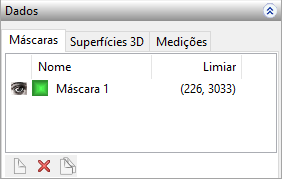
\includegraphics[scale=0.7]{../user_guide_figures/invesalius_screen/painel_mask_manager_pt.png}
\caption{Gerenciamento de dados}
\label{fig:volumetric_data}
\end{figure}

Dentro de cada aba, aparece um painel dividido em linhas e colunas. Em cada linha, a primeira
coluna determina a visualização do elemento listado naquela linha. Isto é, o ícone que
representa um "olho" ativa ou desativa a exibição das máscaras, superfícies ou medições. Caso
um desses elementos esteja em exibição, o ícone da figura \ref{fig:disable_mask} correspondente
a ele também estará visível.

\newpage

\begin{figure}[!htb]
\centering
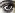
\includegraphics[scale=0.9]{../user_guide_figures/invesalius_screen/eye.jpg}
\caption{Ícone indicativo da visibilidade de elementos}
\label{fig:disable_mask}
\end{figure}

Algumas operações são possíveis sobre os dados. Por exemplo, para excluir um dado, é necessário
primeiro selecionar seu nome, como mostra a figura \ref{fig:selected_mask} e, em seguida, clicar
no atalho que a figura \ref{fig:delete_data} ilustra.

\begin{figure}[!htb]
\centering
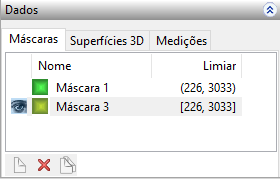
\includegraphics[scale=0.7]{../user_guide_figures/invesalius_screen/painel_selected_mask_pt.png}
\caption{Dado selecionado}
\label{fig:selected_mask}
\end{figure}


\begin{figure}[!htb]
\centering

\includegraphics[scale=0.8]{../user_guide_figures/icons/data_remove.png}
\caption{Excluir dado}
\label{fig:delete_data}
\end{figure}

Para criar uma nova máscara, superfície ou medição, basta clicar no atalho ilustrado na figura
\ref{fig:new_data}, desde que a respectiva aba esteja aberta.

\begin{figure}[!htb]
\centering

\includegraphics[scale=0.8]{../user_guide_figures/icons/data_new.png}
\caption{Novo dado}
\label{fig:new_data}
\end{figure}

Para copiar um dado, basta selecioná-lo e clicar no atalho que a figura \ref{fig:duplicate_data}
ilustra.

\begin{figure}[!htb]
\centering

\includegraphics[scale=0.8]{../user_guide_figures/icons/data_duplicate.png}
\caption{Copiar dado}
\label{fig:duplicate_data}
\end{figure}


\newpage


\section{Máscaras}

Na coluna \textbf{Nome}, são exibidos a cor e o nome atribuídos à máscara. Já a coluna
\textbf{Limiar} exibe o intervalo de valores utilizado para criar a máscara. A figura
\ref{fig:volumetric_data} mostra um exemplo.

\section{Superfícies 3D}

Na coluna \textbf{Nome}, são exibidos a cor e o nome atribuídos à superfície. A coluna 
\textbf{Volume} mostra o volume total da superfície. Por fim, a coluna \textbf{Transparência}
indica o nível de transparência em uso para exibir a superfície. A figura \ref{fig:surface_manager}
traz um exemplo.

\begin{figure}[!htb]
\centering
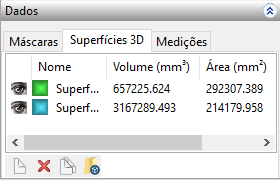
\includegraphics[scale=0.7]{../user_guide_figures/invesalius_screen/painel_volumetric_measures_pt.png}
\caption{Gerenciamento de superfícies}
\label{fig:surface_manager}
\end{figure}

\subsection{Importação de superfície}

É possível importar arquivos do tipo STL, OBJ, PLY e VTP (VTK Polydata File Format) com um projeto do InVesalius ativo, para isso é necessário clicar no ícone que é mostrado na figura~\ref{fig:import_stl}, selecionar (figura~\ref{fig:import_surface}) o formato do arquivo que será importado e depois clicar no \textbf{Abrir}.

\begin{figure}[!htb]
\centering

\includegraphics[scale=0.8]{../user_guide_figures/icons/load_mesh.png}
\caption{Importar Superfície}
\label{fig:import_stl}
\end{figure}

\begin{figure}[!htb]
\centering
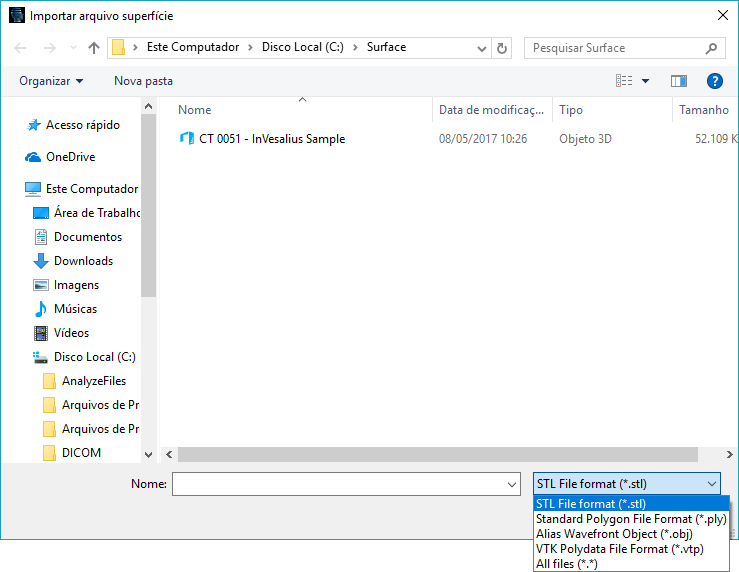
\includegraphics[scale=0.4]{../user_guide_figures/invesalius_screen/import_surface_pt.png}
\caption{Janela para importação de superfície}
\label{fig:import_surface}
\end{figure}

\newpage


\section{Medições}

A aba \textbf{Medições} traz as seguintes informações. A coluna \textbf{Nome} exibe a cor e o
nome atribuídos à medição. A coluna \textbf{Local} exibe onde a medição foi feita (imagem axial,
coronal, sagital ou 3D), e \textbf{Tipo} indica o tipo da medida (linear ou angular). Por último,
a coluna \textbf{Valor} informa a medida propriamente dita. Veja a figura \ref{fig:manager_mensuares}.

\begin{figure}[!htb]
\centering
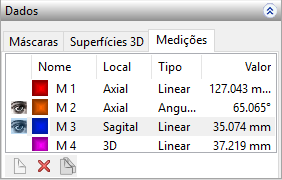
\includegraphics[scale=0.7]{../user_guide_figures/invesalius_screen/painel_measures_manager_pt.png}
\caption{Gerenciamento de medições}
\label{fig:manager_mensuares}
\end{figure}

